\documentclass[conference]{IEEEtran}
% ---------------------------------------------------------
% PACKAGES
% ---------------------------------------------------------
\usepackage{cite}
\usepackage{amsmath,amssymb}
\usepackage{graphicx}
\usepackage{booktabs}
\usepackage{array}
\usepackage{multirow}
\usepackage{url}
\usepackage{xcolor}
\usepackage{tikz}
\usepackage{pgfplots}
\usepackage{float}
\usepackage{enumitem}
\usepackage{placeins}
\usetikzlibrary{
    arrows.meta,
    positioning,
    shapes.geometric,
    shapes.misc,
    fit,
    calc
}
\pgfplotsset{compat=1.18}
% ---------------------------------------------------------
% TEST COUNTS -- single source for every test number in the report.
% Root = tests/ (unittest), Backend = backend/tests (pytest, passing),
% Skipped = the optional PostgreSQL test when TEST_POSTGRES_URL is unset.
% TODO(yash): measured 2026-11-19, PR #1 (engine/net-realisation-rankings):
% backend pytest -q 78 passed, 1 skipped; root unittest 5 OK. Re-measure if
% anything merges after PR #1.
% ---------------------------------------------------------
\newcommand{\TestsRoot}{5}
\newcommand{\TestsBackend}{78}
\newcommand{\TestsSkipped}{1}
\newcommand{\TestsTotal}{83}
% Per-file backend counts (collected test cases incl. parametrized cases;
% they sum to \TestsBackend + \TestsSkipped = 79).
% TODO(yash): measured 2026-11-19, PR #1 -- re-check per-file split on main.
\newcommand{\TestsNetRealisation}{17}
\newcommand{\TestsRankings}{11}
\newcommand{\TestsEngine}{19}
\newcommand{\TestsAPI}{21}
\newcommand{\TestsPortal}{3}
\newcommand{\TestsPresentation}{5}
\newcommand{\TestsHTTP}{1}
\newcommand{\TestsMigrations}{1}
\newcommand{\TestsPostgres}{1}
% ---------------------------------------------------------
% Screenshot slot: shows the PNG if present, otherwise a labelled box.
% ---------------------------------------------------------
\newcommand{\screenshot}[2]{%
\IfFileExists{figures/#1.png}%
{\includegraphics[width=\columnwidth]{figures/#1.png}}%
{\fbox{\parbox[c][3.2cm][c]{0.92\columnwidth}{\centering\small
Screenshot pending: #2\\[2pt]\scriptsize(expected file: \texttt{\detokenize{figures/#1.png}})}}}%
}
% ---------------------------------------------------------
% DOCUMENT
% ---------------------------------------------------------
\begin{document}
% ---------------------------------------------------------
% TITLE
% ---------------------------------------------------------
\title{
MandiWise: A Decision Support System for
Optimal Agricultural Market Selection
}
% ---------------------------------------------------------
% AUTHORS
% ---------------------------------------------------------
\author{
\IEEEauthorblockN{
DHRITY BANSAL\IEEEauthorrefmark{1},
YASHVARDHAN CHAUDHRY\IEEEauthorrefmark{2},
SARTHAK KAUSHIK\IEEEauthorrefmark{3}
}
\IEEEauthorblockA{
Department of Computer Engineering\\
Thapar Institute of Engineering and Technology\\
Punjab, India\\
\IEEEauthorrefmark{1}1024030083,
\IEEEauthorrefmark{2}1024030070,
\IEEEauthorrefmark{3}1024030086
}
}
\maketitle
% ---------------------------------------------------------
% ABSTRACT
% ---------------------------------------------------------
\begin{abstract}
MandiWise is a decision support system that ranks agricultural markets
(mandis) by \textit{net realisation}---the amount a farmer keeps after
commission, market fee, handling and transport---rather than by headline
price, and lets farmers share whole vehicles while each lot stays
identity-preserved. Before building on this idea we tested its premise
against government price data. Across 2,821 same-day cross-sections drawn
from 17,742 price records (two years of history for seven Patiala-district
mandis, plus two days of live Punjab data), the median gross price
dispersion between mandis was 73.1\% and the 25th percentile was 46.7\%,
against a 10\% ``strong'' threshold that was fixed before measuring. The
premise---that nearby mandis do not price alike---therefore holds. The full
product claim---that a farther mandi nets more after real costs---is
\emph{not} yet proven, because the transport rates in the system are
labelled, unsourced placeholders; we can name exactly that piece as the one
that is missing. We implemented two data pullers with documented defences
against silent upstream failures, an exact dynamic-programming
vehicle-packing engine that was checked against brute force and against an
independently written engine (zero cost disagreements in 3,000 randomised
trials), a quantity-proportional cost split that conserves every paisa, a
FastAPI service with a server-enforced pool lifecycle, and \TestsTotal{}
passing automated tests run in continuous integration. This report
describes the design, the evidence, and the limits of both.
\end{abstract}
% ---------------------------------------------------------
% KEYWORDS
% ---------------------------------------------------------
\begin{IEEEkeywords}
Agricultural decision support, mandi selection, net realisation,
farmers, transportation cost, crop pooling, AGMARKNET, market information
system, dynamic programming, open government data.
\end{IEEEkeywords}
% =========================================================
% I. INTRODUCTION
% =========================================================
\section{Introduction}
\label{sec:intro}
Farmers commonly compare mandis by their reported crop prices before
deciding where to sell. The displayed price, however, is not what reaches
the farmer: commission, market fee, loading, weighing, handling and
transport are all deducted along the way, so a mandi with a higher price can
return less money once those costs are counted.

MandiWise was proposed as a decision support system that ranks mandis by
this net amount instead of by headline price, and that lets farmers bound
for the same mandi share a vehicle. This report covers the implementation
phase. Its organising principle is simple: \emph{we tested whether the idea
was true before building on it}. The test confirmed the premise and
identified, precisely, the one input that still stands between the premise
and the product claim.

The contributions of the work are:
\begin{enumerate}[leftmargin=*]
    \item \textbf{A pre-registered validation of the premise}
    (Section~\ref{sec:data}): a price-dispersion measurement over 2,821
    same-day cross-sections, judged against thresholds written down before
    the data was pulled.
    \item \textbf{A data pipeline} of two pullers that defend against
    failure modes which silently corrupt naive ingestion---throttled
    requests that look like empty data, truncated responses and placeholder
    prices (Section~\ref{sec:data}).
    \item \textbf{An exact transport engine}: an unbounded covering dynamic
    programme over integer kilograms and paise, and a largest-remainder cost
    split that conserves every paisa (Section~\ref{sec:engine}), verified by
    brute force and by a differential benchmark against an independently
    written engine (Section~\ref{sec:benchmark}).
    \item \textbf{A pooling backend} with an identity-preserving design, a
    lifecycle enforced on the server, optimistic concurrency control and
    authenticated access (Sections~\ref{sec:pooling}
    and~\ref{sec:security}).
    \item \textbf{A verifiable engineering process}: \TestsTotal{} automated
    tests in continuous integration, an append-only decision log and a
    self-audit backlog of known defects (Sections~\ref{sec:testing}
    and~\ref{sec:process}).
\end{enumerate}
Equally important is what this report does \emph{not} claim. Net
realisation is not proven, transport rates are not real, the liquidity
signal has not been demonstrated on live data, and the multilingual client
is not finished. Section~\ref{sec:limits} lists these limits explicitly.

% =========================================================
% II. PROBLEM STATEMENT
% =========================================================
\section{Problem Statement}
\label{sec:problem}
The primary problem addressed by MandiWise is the difficulty farmers face
in identifying the mandi that provides the highest effective return after
selling and transport costs. Consider a farmer carrying 40 quintals of
potatoes. Suppose Mandi A, 20\,km away, offers INR 1,200 per quintal, while
Mandi B, 60\,km away, offers INR 1,380 per quintal. Mandi B displays the
higher price, but transport and other expenses reduce the difference in
what the farmer actually receives---and whether any advantage survives
depends on those costs. The system therefore aims to answer:
\begin{quote}
\textit{``Which mandi will give the farmer the highest net amount after
considering all relevant costs?''}
\end{quote}
Two further questions follow from it: \textit{is anyone at a given mandi
actually buying this crop}, and \textit{can the farmer share the vehicle
with others going the same way}.

% =========================================================
% III. EXISTING SYSTEMS
% =========================================================
\section{Related and Existing Systems}
\label{sec:existing}
Government market information systems such as AGMARKNET~\cite{agmarknet}
publish daily mandi prices, and the Open Government Data platform exposes
the same feed through an API~\cite{datagov}. The National Agriculture
Market (e-NAM)~\cite{enam} provides an online platform for trading and
price discovery. For research, the CEDA Agri Market Data service of Ashoka
University~\cite{ceda} republishes the AGMARKNET record with historical
depth and daily arrival volumes. All of these report \emph{prices}; none of
them ranks mandis by what an individual farmer nets after his own costs.
Table~\ref{tab:existing} summarises the difference.

\begin{table}[!t]
\caption{Comparison of Existing Approaches and MandiWise}
\label{tab:existing}
\centering
\small
\begin{tabular}{p{0.27\columnwidth} p{0.28\columnwidth} p{0.31\columnwidth}}
\toprule
\textbf{Feature} & \textbf{Existing approach} & \textbf{MandiWise} \\
\midrule
Price information & Market prices & Same prices, each with its reporting date \\
Cost calculation & Mostly manual & Computed by a tested engine \\
Transport cost & Considered separately & Whole-vehicle optimum, in the ranking \\
Net realisation & Not ranked & Primary decision metric \\
Transport pooling & Not central & Identity-preserved vehicle sharing \\
Premise tested on data & --- & Yes (Section~\ref{sec:data}) \\
User roles & General information & Farmer, coordinator, admin \\
\bottomrule
\end{tabular}
\end{table}

% =========================================================
% IV. SYSTEM OVERVIEW AND ARCHITECTURE
% =========================================================
\section{System Overview and Architecture}
\label{sec:architecture}
MandiWise answers three questions, in priority order: \emph{where do I get
the most money} (net-realisation ranking), \emph{is anyone here buying my
crop} (a liquidity signal), and \emph{can I split the vehicle with someone}
(pooling). Five design principles, recorded in the project's architecture
document, shape every component:
\begin{itemize}[leftmargin=*]
    \item \textbf{The engine does exact arithmetic and nothing guesses.}
    Calculations are pure Python with no I/O and no framework imports, so
    they can be tested against hand-computed values.
    \item \textbf{Every number is dated and sourced.} A price is never shown
    without its reporting date, and a rate is never stored without a source
    and an effective date.
    \item \textbf{Rates are data, not code.} Commission, fee, handling and
    vehicle rates belong in configuration tables, not constants.
    \item \textbf{The external API is never called in the request path.}
    Prices are pulled offline and snapshotted.
    \item \textbf{Pool the vehicle, not the produce.}
\end{itemize}

Fig.~\ref{fig:architecture} shows the components as built. Two pullers
fetch prices from the live feed and from the historical CEDA source and
write dated JSON snapshots, which are committed to the repository so that
every analysis runs on the same frozen data. The validation analysis reads
those snapshots directly. A FastAPI~\cite{fastapi} service exposes the
transport, pooling and ranking endpoints; it delegates all arithmetic to
the framework-free engine and persists pools through SQLAlchemy and
Alembic~\cite{sqlalchemy}. Local runs, including every demonstration, use
SQLite; the same migrations are exercised against PostgreSQL~\cite{postgresql}
in continuous integration only. The current user interface is a pair of
server-rendered pages; a React~\cite{react} and Vite~\cite{vite} client
that replaces them has been built and browser-tested, and is pending merge
(Section~\ref{sec:implementation}).

\begin{figure}[!t]
\centering
\resizebox{\columnwidth}{!}{%
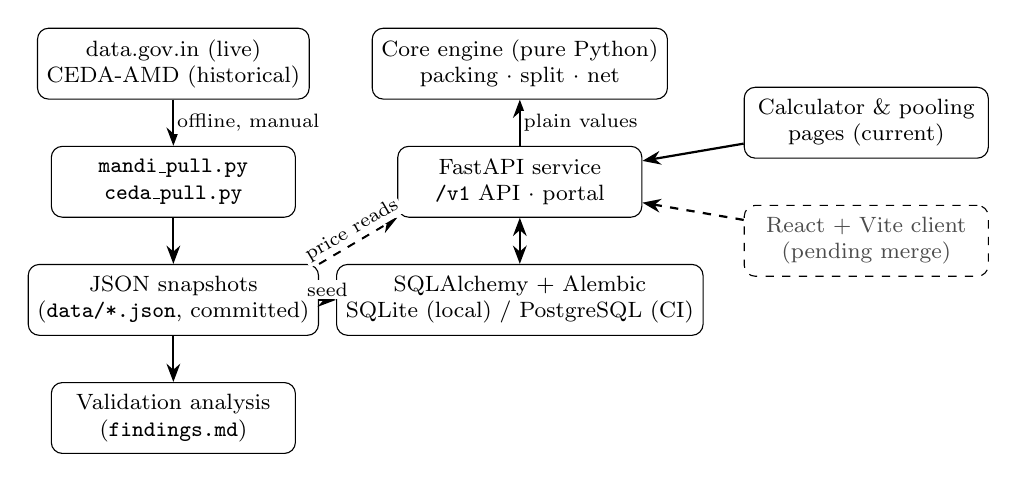
\begin{tikzpicture}[
    box/.style={rectangle, rounded corners, draw, align=center,
        minimum width=31mm, minimum height=9mm, font=\footnotesize},
    planned/.style={box, dashed, text=black!70},
    arrow/.style={-{Stealth}, thick},
    lbl/.style={font=\scriptsize, fill=white, inner sep=1pt}
]
% ingestion column
\node[box] (src) at (0,0) {data.gov.in (live)\\CEDA-AMD (historical)};
\node[box] (pull) at (0,-1.5) {\texttt{mandi\_pull.py}\\\texttt{ceda\_pull.py}};
\node[box] (snap) at (0,-3.0) {JSON snapshots\\(\texttt{data/*.json}, committed)};
\node[box] (ana) at (0,-4.5) {Validation analysis\\(\texttt{findings.md})};
% application column
\node[box] (engine) at (4.4,0) {Core engine (pure Python)\\packing $\cdot$ split $\cdot$ net};
\node[box] (api) at (4.4,-1.5) {FastAPI service\\\texttt{/v1} API $\cdot$ portal};
\node[box] (db) at (4.4,-3.0) {SQLAlchemy + Alembic\\SQLite (local) / PostgreSQL (CI)};
% client column
\node[box] (pages) at (8.8,-0.75) {Calculator \& pooling\\pages (current)};
\node[planned] (react) at (8.8,-2.25) {React + Vite client\\(pending merge)};
% arrows
\draw[arrow] (src) -- node[lbl, right]{offline, manual} (pull);
\draw[arrow] (pull) -- (snap);
\draw[arrow] (snap) -- (ana);
\draw[arrow] (api) -- node[lbl, right]{plain values} (engine);
\draw[{Stealth}-{Stealth}, thick] (api) -- (db);
\draw[arrow] (snap) -- node[lbl, above]{seed} (db);
\draw[arrow] (pages) -- (api);
\draw[arrow, dashed] (react) -- (api);
\draw[arrow, dashed] (snap.north east) -- node[lbl, above, sloped]{price reads} (api.south west);
\end{tikzpicture}%
}
\caption{Components as built. Solid boxes exist and are tested; the dashed
box is built but not yet merged. Pullers run by hand, never inside a user request. The
ranking endpoints read the committed live-feed snapshots once per process
(dashed arrow) until scheduled ingestion writes a price table.}
\label{fig:architecture}
\end{figure}

% =========================================================
% V. DATA PIPELINE AND VALIDATION
% =========================================================
\section{Data Pipeline and Validation}
\label{sec:data}
\subsection{Sources and pullers}
\texttt{mandi\_pull.py} pulls the live AGMARKNET resource from
data.gov.in~\cite{datagov}, paginated by state, and writes each pull as a
dated snapshot. \texttt{ceda\_pull.py} backfills history from
CEDA~\cite{ceda}, including daily arrival volumes. CEDA is free for
non-commercial use only, with attribution; it would have to be re-sourced
if MandiWise were ever commercialised. Neither puller runs on a schedule
yet: both are manual commands, and scheduled ingestion is future work.

The corpus analysed here is the committed data as of 2026-09-17. The
historical part has 16,907 rows from 2023-10-02 to 2025-10-30, covering 7
Patiala-district mandis (Dudhansadhan, Ghanaur, Nabha, Patiala, Patran,
Rajpura, Samana) and 8 vegetables (potato, onion, tomato, green chilli,
brinjal, cauliflower, bhindi, cucumber); 92\% of these rows also carry
arrival volumes. The live part has 836 rows from 50 Punjab mandis over two
days, 2026-09-04 and 2026-09-07. After de-duplication the corpus holds
17,742 rows. The two parts cover disjoint time windows and are never
compared with each other; because grade is part of the grouping key and
CEDA carries no grades, cross-source contamination is structurally
impossible.

\subsection{Method}
The measurements and their reading thresholds were written into the
project's working file \emph{before} any data was pulled:
\begin{itemize}[leftmargin=*]
    \item \textbf{Price spread.} For each date and commodity, across mandis
    reporting the same commodity, variety and grade, compute
    $(\max \text{modal} - \min \text{modal}) / \min \text{modal}$. Groups
    with fewer than 3 reporting mandis are discarded. A median above 10\%
    reads as strong, 4--10\% as conditional, and below 3\% as failure of
    the arbitrage premise.
    \item \textbf{Liquidity.} For each (mandi, commodity) pair, count
    reporting days in a trailing 30-day window.
\end{itemize}
A weak spread was declared in advance to be a finding, not a failure: the
product would then pivot towards liquidity and pooling.

\subsection{Results}
Table~\ref{tab:validation} and Fig.~\ref{fig:dispersion} give the results.
The median dispersion across 2,821 comparable groups is 73.1\%, and even
the 25th percentile, 46.7\%, sits far above the 10\% threshold. The
pre-declared verdict is \textbf{strong}, and the pivot contingency is not
triggered.

\begin{table}[!t]
\caption{Validation Results (corpus as of 2026-09-17)}
\label{tab:validation}
\centering
\small
\setlength{\tabcolsep}{4pt}
\begin{tabular}{p{0.58\columnwidth} r}
\toprule
\textbf{Measure} & \textbf{Value} \\
\midrule
\multicolumn{2}{l}{\textit{Corpus}} \\
Historical rows (CEDA), 2023-10-02 to 2025-10-30 & 16,907 \\
Live rows (data.gov.in), 50 mandis, 2 days & 836 \\
Total after de-duplication & 17,742 \\
\midrule
\multicolumn{2}{l}{\textit{Price spread}} \\
Comparable groups ($\geq$3 mandis) & 2,821 \\
25th percentile dispersion & 46.7\% \\
\textbf{Median dispersion} & \textbf{73.1\%} \\
75th percentile dispersion & 113.9\% \\
Verdict against the $>$10\% threshold & Strong \\
\midrule
\multicolumn{2}{l}{\textit{Liquidity, 2025-10-01 to 2025-10-30 (historical)}} \\
Market--commodity pairs & 45 \\
Median reporting days & 21 of 30 \\
25th / 75th percentile & 16 / 23 \\
Active / intermittent / sparse pairs & 27 / 17 / 1 \\
Live liquidity (2 days observed) & not measurable \\
\bottomrule
\end{tabular}
\end{table}

\begin{figure}[!t]
\centering
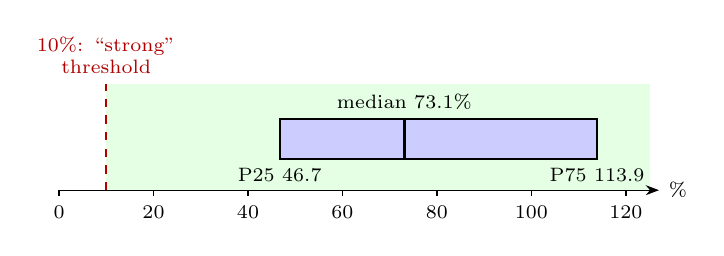
\begin{tikzpicture}[x=0.06cm, y=1cm, font=\scriptsize]
\fill[green!10] (10,0) rectangle (125,1.35);
\draw[-{Stealth}] (0,0) -- (127,0) node[right] {\%};
\foreach \x in {0,20,40,60,80,100,120}
    \draw (\x,0) -- (\x,-0.08) node[below] {\x};
\draw[dashed, thick, red!70!black] (10,0) -- (10,1.35)
    node[above, align=center] {10\%: ``strong''\\threshold};
\draw[thick, fill=blue!20] (46.7,0.4) rectangle (113.9,0.9);
\draw[very thick] (73.1,0.4) -- (73.1,0.9);
\node[above] at (73.1,0.9) {median 73.1\%};
\node[below] at (46.7,0.4) {P25 46.7};
\node[below] at (113.9,0.4) {P75 113.9};
\end{tikzpicture}

\IfFileExists{figures/ceda_logo.png}{%
\vspace{2pt}\hfill\includegraphics[height=0.5cm]{figures/ceda_logo.png}}{}
\caption{Interquartile range of same-day price dispersion across 2,821
cross-sections (box) against the pre-declared 10\% threshold. Historical
data: CEDA Agri Market Data (CEDA-AMD), Centre for Economic Data \&
Analysis, Ashoka University; live data: AGMARKNET via data.gov.in, Ministry
of Agriculture \& Farmers Welfare.}
\label{fig:dispersion}
\end{figure}
% TODO(yash): CEDA requires its logo on published visuals derived from its
% data. Save it as report/figures/ceda_logo.png and it appears in Fig. 2.

\subsection{What the result does and does not establish}
The result establishes that \textbf{prices across nearby mandis do not
cluster}: the premise on which the product rests is real and large. It does
\textbf{not} establish that a farther mandi nets more. Dispersion is a
\emph{gross} spread; the product claim concerns the spread \emph{after}
commission, market fee, handling and transport. A 73.1\% median is a wide
cushion for those costs, but it has not been tested against real rates.
The historical comparisons are also confined to one district, tighter than
the roughly 100\,km radius the product targets; a wider radius would be
expected to widen spreads, but that is an expectation, not a measurement.

On liquidity, most pairs trade on most days, yet 18 of the 45 pairs
(intermittent plus sparse) are not active. ``Is anyone buying my crop this
week'' is therefore a question separate from ``where is the price
highest''. The 60\%/20\% cut-offs behind the active, intermittent and
sparse labels are a provisional reading aid, not a sourced threshold. With
only two live days captured, liquidity cannot yet be judged on live data at
all; that requires daily pulls to accumulate.

\subsection{Data-quality findings}
Each of the following was found by checking rather than by assuming, and
each would silently corrupt a naive pipeline:
\begin{enumerate}[leftmargin=*]
    \item \textbf{Placeholder prices.} One mandi (Patti APMC) reported modal
    prices of INR 0.08--32.90 on both live pull days, against real prices
    starting near INR 200. A floor of INR 50 per quintal rejects and logs
    these rows; they are never corrected or estimated. Without the floor, a
    single green-chilli comparison inflated to a meaningless 3,807,900\%
    dispersion. The median is unaffected; the damage is to individual
    comparisons.
    \item \textbf{Inconsistent commodity names.} Of the 57 commodity names
    seen in the live feed, 40 match CEDA exactly; roughly 30\% do not. Two
    names could not be mapped and were left unmapped rather than
    guessed.
    \item \textbf{Mixed scripts.} The live feed carries a row with a
    Devanagari name, which breaks any pipeline that assumes ASCII.
    \item \textbf{Throttling that looks like absence.} CEDA can answer a
    throttled request with HTTP 200 and an empty body, so every empty
    response is re-probed before it is believed. Responses are capped at
    1,000 rows, so a full response is treated as truncated and the date
    range is split recursively. \texttt{Retry-After} arrives in
    milliseconds rather than seconds.
    \item \textbf{A silent gateway filter.} The data.gov.in gateway drops
    requests whose User-Agent contains ``python''---no error, just a hang.
    Both pullers send an explicit project User-Agent.
    \item \textbf{Insufficient validation rule.} Of the 17,742 rows, 17,737
    pass the architecture's validation rule (date parses, modal $>0$,
    $\min \le \text{modal} \le \max$), yet 19 of those still have a modal
    price below INR 10 per quintal. The rule is necessary but not
    sufficient, which is why the price floor exists.
\end{enumerate}

% =========================================================
% VI. CORE ENGINE
% =========================================================
\section{Core Engine: Net Realisation, Vehicle Packing and Cost Split}
\label{sec:engine}
The engine is a plain Python module with no database, network or framework
imports. Quantities are held as integer kilograms and money as integer
paise, so no floating-point rounding enters any total. A vehicle's trip
price, base cost plus per-km rate times distance, is computed by a single
engine function and rounded once, half-up, to a whole paisa.

\subsection{Net realisation}
For a lot of $Q$ quintals at a mandi reporting modal price $P$ per quintal,
with commission rate $c$, market-fee rate $f$ and handling charge $h$ per
quintal:
\begin{align}
G &= P \cdot Q \label{eq:gross}\\
C &= c \cdot G \label{eq:commission}\\
F &= f \cdot G \label{eq:fee}\\
H &= h \cdot Q \label{eq:handling}
\end{align}
Transport is procured in whole vehicles, not in proportion to the load.
For a lot carried over distance $d$, where vehicle class $i$ has capacity
$\kappa_i$ and trip cost $\beta_i + \gamma_i d$ (a base cost plus a per-km
rate), transport cost is the least-cost allocation of whole vehicles
sufficient to carry the lot:
\begin{equation}
T(Q,d) = \min_{\mathbf{n} \in \mathcal{N}(Q)}
\; \sum_{i} n_i \left( \beta_i + \gamma_i d \right)
\label{eq:transport}
\end{equation}
\begin{equation}
\mathcal{N}(Q) = \Big\{ \mathbf{n} \in \mathbb{Z}_{\geq 0}^{k}
\; : \; \textstyle\sum_{i} n_i \kappa_i \geq Q \Big\}
\label{eq:feasible}
\end{equation}
The net realisation is then
\begin{equation}
N = G - C - F - H - T(Q,d).
\label{eq:net}
\end{equation}
Because a modal price is a typical outcome rather than a guarantee,
(\ref{eq:net}) is also evaluated at the reported minimum and maximum prices,
giving a range $[N_{\min}, N_{\max}]$ that is shown alongside $N$.

The market-fee term $F$ and the range were missing from the first engine
written for the project; an audit found that every net figure it reported
was therefore overstated by $f \cdot G$. Net realisation was then rebuilt
in the canonical engine in integer paise and kilograms, with the rates $c$
and $f$ held in basis points. Each deduction in (\ref{eq:commission})--(\ref{eq:handling})
is rounded half-up to the paisa on its own and $N$ is taken from the
rounded components, so a displayed breakdown always sums exactly to the
displayed net---a test checks this at four fee rates. A net below zero is
reported as it is, never clamped. The rebuilt module is exposed through a
ranking API (\texttt{POST /v1/rankings}, with \texttt{GET /v1/markets} for
the latest dated observations and \texttt{GET /v1/commodities}). A price
more than two days old is flagged as stale and still shown with its date,
never hidden or silently substituted; the threshold is recorded in the
decision log.

The market-fee \emph{term} is therefore implemented, but its \emph{rate}
is not sourced. Rather than invent one, the ranking API runs with a fee
rate of zero, read from a rate file labelled as a placeholder, and every
response warns that net realisation is overstated by the fee. The term
matters: a test shows that on the proposal's original worked example, a 3\%
fee charged at the distant mandi alone (INR 1,656) lowers its net to INR
41,136, below the local mandi's INR 41,880, and flips the ranking. Sourcing
the fee rate is therefore part of the same blocking step as sourcing
transport rates (Section~\ref{sec:limits}).

\subsection{Vehicle packing as dynamic programming}
The integrality of $\mathbf{n}$ makes cost per quintal a step function of
load: it jumps when a load crosses a capacity boundary and falls as the
engaged vehicle fills (Fig.~\ref{fig:step}). That non-linearity is why a
small lot is expensive to move and the direct reason pooling helps.

The engine solves (\ref{eq:transport}) exactly as an unbounded covering
problem~\cite{martello} over integer kilograms. Let $\pi_i$ be the trip
cost of class $i$ in paise. Each remaining load $q = 1,\dots,Q$ is assigned
a score triple $\mathbf{s}(q)$ = (cost, vehicle count, capacity provided):
\begin{equation}
\mathbf{s}(q) = \operatorname*{lexmin}_{i}\;
\Big[\mathbf{s}\big(\max(0,\,q-\kappa_i)\big) + (\pi_i,\,1,\,\kappa_i)\Big],
\label{eq:dp}
\end{equation}
with $\mathbf{s}(0) = (0,0,0)$. Lexicographic comparison implements the tie-break
policy: least cost, then fewest vehicles, then least capacity; remaining
ties are settled by vehicle code so the result is deterministic. The fleet
is recovered by back-tracking the stored choice. The algorithm runs in
$O(Qk)$ time and $O(Q)$ memory for $Q$ kilograms and $k$ vehicle classes.
Inputs are bounded to 0.01--1,000 quintals in whole kilograms and 1--12
vehicle classes, and a vehicle with zero trip cost is rejected.

The DP is verified in the test suite against an exhaustive search over 100
randomly generated three-class fleets, comparing the full score triple, and
against hand-chosen capacity boundaries (Fig.~\ref{fig:step}).

\begin{figure}[!t]
\centering
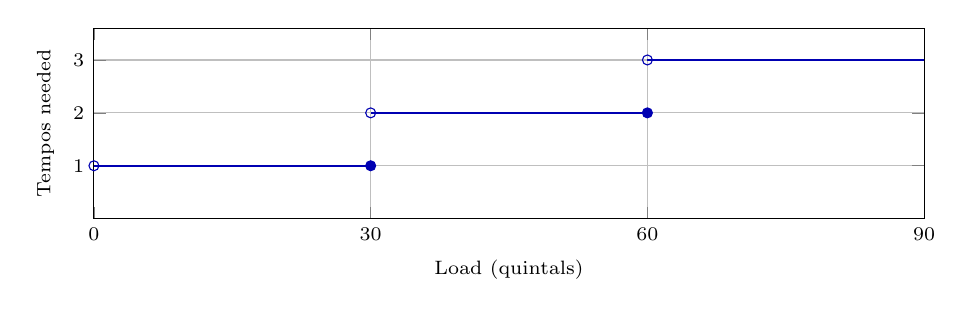
\begin{tikzpicture}
\begin{axis}[
    width=\columnwidth, height=4.0cm,
    xmin=0, xmax=90, ymin=0, ymax=3.6,
    xtick={0,30,60,90}, ytick={1,2,3},
    xlabel={Load (quintals)}, ylabel={Tempos needed},
    tick label style={font=\scriptsize},
    label style={font=\scriptsize},
    grid=major
]
\addplot[thick, blue!70!black, no marks] coordinates {(0,1) (30,1)};
\addplot[thick, blue!70!black, no marks] coordinates {(30,2) (60,2)};
\addplot[thick, blue!70!black, no marks] coordinates {(60,3) (90,3)};
\addplot[only marks, mark=*, mark size=1.8pt, blue!70!black]
    coordinates {(30,1) (60,2)};
\addplot[only marks, mark=o, mark size=1.8pt, blue!70!black,
    mark options={fill=white}] coordinates {(0,1) (30,2) (60,3)};
\end{axis}
\end{tikzpicture}
\caption{Vehicle count is a step function of load (single 30-quintal tempo
class). The boundaries are asserted in \texttt{test\_capacity\_boundaries}:
29.99, 30.00, 30.01, 60.00 and 60.01 quintals need 1, 1, 2, 2 and 3 tempos.}
\label{fig:step}
\end{figure}

\subsection{Cost split by largest remainder}
When participants $j$ with quantities $q_j$ share a pooled trip of cost
$K = T(\sum_j q_j, d)$ paise, each is charged
\begin{equation}
s_j = \left\lfloor \frac{K\, q_j}{\sum_{\ell} q_\ell} \right\rfloor
+ \delta_j, \qquad \sum_j s_j = K,
\label{eq:split}
\end{equation}
where $\delta_j \in \{0,1\}$ hands the $K - \sum_j \lfloor\cdot\rfloor$
leftover paise to the participants with the largest remainders, ties broken
by participant identifier. This is the largest-remainder (Hamilton)
apportionment~\cite{balinski}: every share is within one paisa of its exact
proportion and the shares sum to the pooled cost exactly, with no rounding
leak. For example, 100 paise split three equal ways gives 34, 33 and 33.

The split is by \textbf{quantity}, never by sale value: everyone pays for
the space they occupy, so a farmer with premium produce does not subsidise
anyone. Savings are not distributed; they \emph{follow} from the split. A
participant's saving is
\begin{equation}
\sigma_j = T(q_j, d) - s_j,
\label{eq:saving}
\end{equation}
his solo transport cost minus his share. A group saving does not guarantee
that every member saves---a tested counter-example exists---so the
lifecycle refuses to lock a pool in which any $\sigma_j < 0$
(Section~\ref{sec:pooling}).

% =========================================================
% VII. POOLING DESIGN AND LIFECYCLE
% =========================================================
\section{Pooling Design and Lifecycle}
\label{sec:pooling}
\subsection{Identity-preserved pooling}
MandiWise pools \emph{transport}, not \emph{produce}. Each farmer's lot is
separately bagged, weighed and auctioned under his own name; three farmers
sharing a truck are three lots in one vehicle, not one blended lot, so a
premium-grade lot still earns a premium-grade price. Three safeguards
follow: each member declares variety, grade and condition when requesting
to join; the coordinator, who is physically present, may decline any
request; and the cost split is by quantity. The platform does not
adjudicate quality disputes; it keeps the record of what each member
declared.

\subsection{Worked pooling example}
Fig.~\ref{fig:pooling} shows the pooling example used throughout the test
suite, under the project's single placeholder rate card (tempo: 30
quintals, INR 1,000 plus INR 10 per km; truck: 100 quintals, INR 2,500 plus
INR 20 per km). At 60\,km a tempo trip costs INR 1,600 and a truck trip INR
3,700. One farmer with 40 quintals needs two tempos, INR 3,200; two such
farmers travelling separately pay INR 6,400 between them. Pooled, their 80
quintals fit one truck for INR 3,700, or INR 1,850 each---a saving of INR
1,350 each and INR 2,700 in total. A third 40-quintal lot would make 120
quintals, which a 100-quintal truck cannot hold: the engine then selects a
truck plus a tempo for INR 5,300, a case asserted in the tests.

\begin{figure}[!t]
\centering
\resizebox{\columnwidth}{!}{%
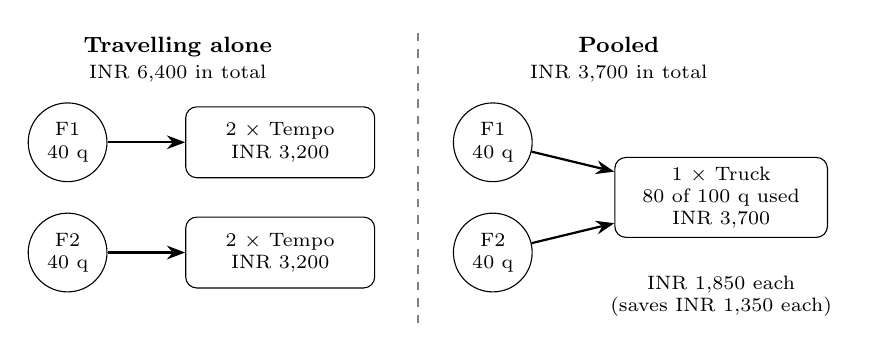
\begin{tikzpicture}[
    farmer/.style={circle, draw, minimum size=10mm, align=center,
        font=\scriptsize, inner sep=0pt},
    vehicle/.style={rectangle, rounded corners, draw, align=center,
        minimum width=24mm, minimum height=9mm, font=\scriptsize},
    arrow/.style={-{Stealth}, thick},
    title/.style={font=\footnotesize\bfseries, align=center}
]
% travelling alone
\node[title] at (1.4,1.75) {Travelling alone\\\normalfont\scriptsize INR 6,400 in total};
\node[farmer] (f1) at (0,0.7) {F1\\40 q};
\node[farmer] (f2) at (0,-0.7) {F2\\40 q};
\node[vehicle] (v1) at (2.7,0.7) {2 $\times$ Tempo\\INR 3,200};
\node[vehicle] (v2) at (2.7,-0.7) {2 $\times$ Tempo\\INR 3,200};
\draw[arrow] (f1) -- (v1);
\draw[arrow] (f2) -- (v2);
% divider
\draw[dashed, gray] (4.45,-1.6) -- (4.45,2.1);
% pooled
\node[title] at (7.0,1.75) {Pooled\\\normalfont\scriptsize INR 3,700 in total};
\node[farmer] (g1) at (5.4,0.7) {F1\\40 q};
\node[farmer] (g2) at (5.4,-0.7) {F2\\40 q};
\node[vehicle, minimum width=27mm] (truck) at (8.3,0)
    {1 $\times$ Truck\\80 of 100 q used\\INR 3,700};
\draw[arrow] (g1) -- (truck);
\draw[arrow] (g2) -- (truck);
\node[font=\scriptsize, align=center] at (8.3,-1.25)
    {INR 1,850 each\\(saves INR 1,350 each)};
\end{tikzpicture}%
}
\caption{Pooling two 40-quintal lots over 60\,km under the placeholder rate
card. Each lot keeps its owner's identity; only the vehicle is shared. All
figures are asserted in \texttt{test\_engine.py} and
\texttt{test\_presentation.py}. Rates are PLACEHOLDER, UNSOURCED.}
\label{fig:pooling}
\end{figure}

\subsection{Lifecycle}
A pool moves through the states of Fig.~\ref{fig:lifecycle}. The allowed
transitions are enforced in the service layer, so an invalid move is
rejected by the server rather than merely hidden in the user interface.
The database's CHECK constraint restricts the \emph{values} a state can
take; it does not encode the transitions, which live in code. Only the
pool's own coordinator may move it, and each move must quote the pool's
current \texttt{version}. The guards are:
\begin{enumerate}[label=(\alph*), leftmargin=*]
    \item \textbf{Lock} (OPEN$\rightarrow$LOCKED): the travel date is not
    in the past; no join request is still PENDING; at least one member is
    APPROVED; and no member's share exceeds what he would pay travelling
    alone. The cost split is then frozen into the pool record.
    \item \textbf{Dispatch} (LOCKED$\rightarrow$DISPATCHED): a transport
    arrangement reference must be recorded.
    \item \textbf{Settle} (DISPATCHED$\rightarrow$SETTLED): an outcome note
    is required.
    \item \textbf{Cancel} (from OPEN or LOCKED): a cancellation note is
    required.
\end{enumerate}
Every membership change and transition increments the pool's version
column, which the ORM uses for optimistic concurrency control: two
coordinators' writes against the same snapshot cannot both commit, and a
stale client receives a \texttt{version\_conflict} error and must reload.
Every action also writes an event row, giving each pool an audit trail.

\begin{figure}[!t]
\centering
\resizebox{\columnwidth}{!}{%
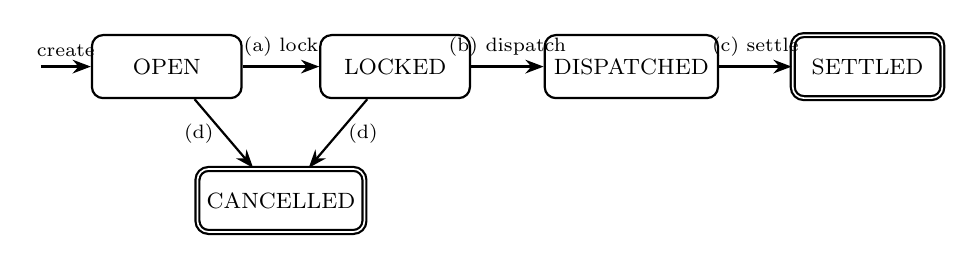
\begin{tikzpicture}[
    st/.style={rectangle, rounded corners, draw, thick, align=center,
        minimum width=19mm, minimum height=8mm, font=\footnotesize},
    final/.style={st, double},
    arrow/.style={-{Stealth}, thick},
    lbl/.style={font=\scriptsize}
]
\node[st] (open) at (0,0) {OPEN};
\node[st] (locked) at (2.9,0) {LOCKED};
\node[st] (disp) at (5.9,0) {DISPATCHED};
\node[final] (settled) at (8.9,0) {SETTLED};
\node[final] (cancel) at (1.45,-1.7) {CANCELLED};
\draw[arrow] (-1.6,0) -- node[lbl, above]{create} (open);
\draw[arrow] (open) -- node[lbl, above]{(a) lock} (locked);
\draw[arrow] (locked) -- node[lbl, above]{(b) dispatch} (disp);
\draw[arrow] (disp) -- node[lbl, above]{(c) settle} (settled);
\draw[arrow] (open) -- node[lbl, left]{(d)} (cancel);
\draw[arrow] (locked) -- node[lbl, right]{(d)} (cancel);
\end{tikzpicture}%
}
\caption{Pool lifecycle as enforced by the service layer. Double borders
mark terminal states. Letters refer to the guards listed in the text.}
\label{fig:lifecycle}
\end{figure}

\subsection{Roles}
Table~\ref{tab:roles} lists the three roles. The design records Pool
Coordinator as a \emph{permission} on a farmer account, not a separate user
type. The current implementation models it as a mutually exclusive role,
and the self-service portal registers every user as a coordinator so that
farmers can organise their own trips. This contradicts the recorded
decision; it is logged as a task rather than silently carried.

\begin{table}[!t]
\caption{User Roles and Responsibilities}
\label{tab:roles}
\centering
\small
\begin{tabular}{p{0.22\columnwidth} p{0.68\columnwidth}}
\toprule
\textbf{Role} & \textbf{Responsibilities}\\
\midrule
Farmer &
View mandi rankings, declare a lot and request to join a pool, see only
his own share, withdraw, and use the pool's group chat once approved.\\
Pool Coordinator &
Post a trip, review join requests, monitor approved load against the
pool's limit, lock the cost split, record the transport arrangement and the
outcome. Designed as a permission; currently a role (logged task).\\
Administrator &
Maintain the catalogue of locations, routes and rate cards, each with a
source and an effective period.\\
\bottomrule
\end{tabular}
\end{table}

% =========================================================
% VIII. DATABASE DESIGN
% =========================================================
\section{Database Design}
\label{sec:database}
Table~\ref{tab:db} lists the tables as defined in the ORM models and
created by two Alembic migrations. A migration test checks that the
migrated schema matches the models exactly and that downgrade removes it.
Provenance is part of the schema, not a comment: routes and rate cards
cannot be stored without a source string and an effective period, and a
rate card carries an explicit \texttt{is\_demo} flag that makes the API
attach a ``synthetic demonstration rates'' warning to every quote it
produces.

\begin{table}[!t]
\caption{Persisted Tables (prefix \texttt{transport\_} omitted)}
\label{tab:db}
\centering
\scriptsize
\setlength{\tabcolsep}{3pt}
\begin{tabular}{p{0.24\columnwidth} p{0.68\columnwidth}}
\toprule
\textbf{Table} & \textbf{Key attributes and constraints}\\
\midrule
\texttt{users} & id, name, role $\in$ \{farmer, coordinator, admin\}, active\\
\texttt{portal\_accounts} & user (PK, FK), unique username, scrypt password hash, village\\
\texttt{locations} & name, kind $\in$ \{origin, mandi\}, state, district, source; unique (name, kind, state, district)\\
\texttt{routes} & origin, destination, distance in metres ($>0$), source, effective from/until\\
\texttt{rate\_cards} & route endpoints, source, effective from/until, \texttt{is\_demo}, vehicle classes (JSON)\\
\texttt{pools} & coordinator, route, rate card, travel date, commodity, pickup point, maximum load (kg), state, version, frozen quote (JSON), transport reference\\
\texttt{pool\_members} & pool, user, quantity (kg), variety, grade, condition, status $\in$ \{PENDING, APPROVED, REJECTED, WITHDRAWN\}; unique (pool, user)\\
\texttt{pool\_events} & pool, actor, action, detail (JSON), timestamp --- audit trail\\
\texttt{portal\_messages} & pool, author, body, timestamp --- group chat\\
\bottomrule
\end{tabular}
\end{table}

Not every entity in the architecture exists yet. Price observations remain
in the committed JSON snapshots rather than a \texttt{price\_record} table:
the ranking API loads them once per process and validates them on load,
rejecting a modal price below the INR 50 floor or outside its own reported
minimum and maximum. Commission, fee and handling rates live in a
placeholder rate file with a source note and an effective date, not yet
in a dated \texttt{rate\_config} table; and there is no precomputed
distance matrix, so distances are entered by the user. These are planned
(Section~\ref{sec:future}).

% =========================================================
% IX. ILLUSTRATIVE COMPARISON
% =========================================================
\section{Illustrative Mandi Comparison}
\label{sec:comparison}
Table~\ref{tab:comparison} and Fig.~\ref{fig:netchart} reproduce, exactly,
the output of the project's \texttt{demo.py} for the 40-quintal potato
example of Section~\ref{sec:problem}. The prices, distances, 4\%
commission and INR 30 per quintal handling come from a file that labels
itself ``illustrative project example---not government data''; the
transport rates are the placeholder card of Section~\ref{sec:pooling}. The
program prints the placeholder warning before any figure. This is a
demonstration of the \emph{mechanism}, not a measured outcome.

\begin{table}[!t]
\caption{Illustrative Comparison, 40 q Potato (output of \texttt{demo.py};
rates PLACEHOLDER, UNSOURCED)}
\label{tab:comparison}
\centering
\small
\begin{tabular}{lrr}
\toprule
\textbf{Parameter} & \textbf{Mandi A (local)} & \textbf{Mandi B (distant)}\\
\midrule
Distance & 20 km & 60 km\\
Modal price / quintal & INR 1,200 & INR 1,380\\
Gross revenue & INR 48,000 & INR 55,200\\
Commission (4\%) & INR 1,920 & INR 2,208\\
Handling (INR 30/q) & INR 1,200 & INR 1,200\\
Transport & INR 2,400 & INR 3,200\\
\quad vehicles & 2 $\times$ Tempo & 2 $\times$ Tempo\\
\textbf{Net realisation} & \textbf{INR 42,480} & \textbf{INR 48,592}\\
\textbf{Rank} & 2 & 1\\
\bottomrule
\end{tabular}
\end{table}

\begin{figure}[!t]
\centering
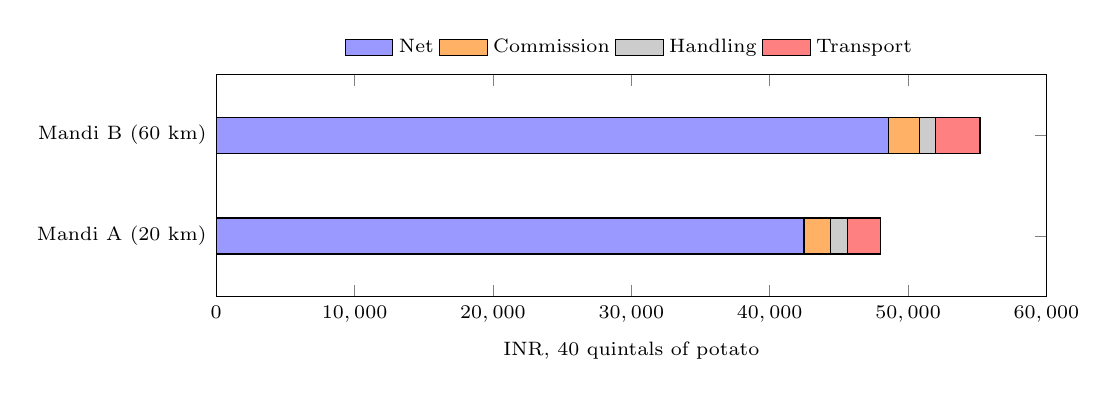
\begin{tikzpicture}
\begin{axis}[
    xbar stacked,
    bar width=13pt,
    width=\columnwidth, height=4.4cm,
    xmin=0, xmax=60000,
    ymin=0.4, ymax=2.6,
    ytick={1,2},
    yticklabels={{Mandi A (20 km)},{Mandi B (60 km)}},
    xlabel={INR, 40 quintals of potato},
    scaled x ticks=false,
    xticklabel style={/pgf/number format/1000 sep={,}},
    tick label style={font=\scriptsize},
    label style={font=\scriptsize},
    legend style={at={(0.5,1.03)}, anchor=south, legend columns=4,
        font=\scriptsize, draw=none},
    area legend
]
\addplot[fill=blue!40, draw=black] coordinates {(42480,1) (48592,2)};
\addplot[fill=orange!60, draw=black] coordinates {(1920,1) (2208,2)};
\addplot[fill=gray!40, draw=black] coordinates {(1200,1) (1200,2)};
\addplot[fill=red!50, draw=black] coordinates {(2400,1) (3200,2)};
\legend{Net, Commission, Handling, Transport}
\node[font=\scriptsize] at (axis cs:21240,1) {42,480};
\node[font=\scriptsize] at (axis cs:24296,2) {48,592};
\end{axis}
\end{tikzpicture}
\caption{Where each mandi's gross revenue goes, from Table~\ref{tab:comparison}.
Bar length is gross revenue. Rates are PLACEHOLDER, UNSOURCED; the
market-fee term is absent from this calculation.}
\label{fig:netchart}
\end{figure}

Four observations keep this example honest. First, the backend engine
independently reproduces both transport figures and the same
2 $\times$ Tempo fleet, even with the truck also available
(Section~\ref{sec:benchmark}). Second, the rebuilt ranking API reproduces
both nets, INR 48,592 and INR 42,480, in its tests; given test-fixture
minimum and maximum prices of INR 1,300 and INR 1,450 for the distant
mandi, it reports a range of INR 45,520--51,280 around the INR 48,592
figure. Third, the original proposal ran the same
example with a base-cost-free rate card and obtained INR 41,880 against
INR 42,792; the size of Mandi B's advantage depends heavily on the rate
card, which is exactly why sourced rates are the blocking input. Fourth,
\texttt{demo.py} runs the first engine, which has no market-fee term, and
the ranking API runs with a fee rate of zero because none is sourced, so
neither figure includes a fee. Using \emph{assumed} fee rates purely as
probes---not Punjab's actual fee~\cite{punjabact}---the ranking in this
example survives: at an assumed 2\% the nets become INR 47,488 and INR
41,520. That is one two-row example, not a general guarantee; under the
proposal's original rate card a 3\% fee does flip the ranking
(Section~\ref{sec:engine}).

% =========================================================
% X. IMPLEMENTATION AND USER INTERFACE
% =========================================================
\section{Implementation and User Interface}
\label{sec:implementation}
\subsection{Technology and status}
The backend is Python 3.12 with FastAPI~\cite{fastapi}, Pydantic for
request validation, SQLAlchemy and Alembic~\cite{sqlalchemy}, PyJWT and
Uvicorn; the engine and pullers use only the standard library. Tests run
under pytest and unittest, linting under ruff, and continuous integration
on GitHub Actions. Table~\ref{tab:status} states plainly what is built,
what is partial and what is planned.

\begin{table}[!t]
\caption{Implementation Status}
\label{tab:status}
\centering
\scriptsize
\setlength{\tabcolsep}{3pt}
\begin{tabular}{p{0.42\columnwidth} p{0.14\columnwidth} p{0.34\columnwidth}}
\toprule
\textbf{Component} & \textbf{Status} & \textbf{Where / note}\\
\midrule
Live and historical pullers & Built & \texttt{mandi\_pull.py}, \texttt{ceda\_pull.py}; manual runs\\
Premise validation analysis & Built & \texttt{research/findings.md}\\
Vehicle packing (DP) & Built & \texttt{engine.py}\\
Cost split (largest remainder) & Built & \texttt{engine.py}\\
Net realisation with fee and range & Built & \texttt{engine.py}; fee rate unsourced (0)\\
Ranking API & Built & \texttt{/v1/rankings}, \texttt{/v1/markets}; reads snapshots\\
Transport and pool API & Built & \texttt{/v1} (FastAPI)\\
Pool lifecycle, concurrency, audit & Built & \texttt{services.py}\\
Accounts, sessions, CSRF checks & Built & local prototype only\\
Calculator and pooling pages & Built & server-rendered; English only\\
React + Vite client & Partial & in progress\\
Internationalisation (13 locales) & Partial & scope decided; en/hi/pa first\\
Real transport rates & Planned & blocking input\\
Sourced commission and fee rates & Planned & probes only so far\\
Scheduled ingestion & Planned & pullers are manual\\
Liquidity signal in the product & Planned & historical analysis only\\
Distance matrix & Planned & distances entered by user\\
Public deployment & Planned & no live URL yet\\
\bottomrule
\end{tabular}
\end{table}

\subsection{User interface}
Two server-rendered pages exist today and are what a demonstration shows.
The transport calculator takes each farmer's quantity, a road distance and
editable vehicle prices, and shows the cheapest vehicle combination, each
farmer's solo and shared cost, and a plain-language ``how we calculated
it'' expansion of the arithmetic; it carries a visible ``classroom
example'' label. The farmer pooling portal supports accounts, posting a
trip, discovering trips, requesting to join with a declared lot,
approval, a cost estimate and a group chat restricted to approved members.

These pages work but look unfinished, and the earlier review of the project
said so. A React~\cite{react} client built with Vite~\cite{vite} has
therefore been written to replace them. It uses hash routes for an
overview, a mandi price explorer, the transport calculator, trip
discovery, own trips, trip creation, trip detail and a data/help page,
with a desktop sidebar and a responsive mobile layout. It calls the
existing REST endpoints for accounts, calculation, pool membership,
quotes, lifecycle transitions and chat, sending the custom request
header and the expected record version on every write. It performs no
vehicle optimisation, cost allocation or net-realisation arithmetic of its
own; the only conversions it makes are for display (kilograms to quintals,
paise-formatted rupees). Its development server proxies the API on the same
origin, so the backend's cookie and cross-origin checks remain in force.

Verification of the client was a production build, four unit tests of the
display helpers, and a headless-browser run against an isolated test
database. That run covered desktop and a 390-pixel mobile viewport,
registration, trip creation, approval, quoting, chat, locking, and
persistence after reload. It also confirmed that an unauthenticated chat
request is rejected (401) and that a cross-origin write is rejected (403).
Dispatch, settlement, cancellation, rejection and withdrawal are wired to
the API but were not exercised in that run.

The mandi explorer currently lists dated observations from one committed
snapshot. It does not yet show net-realisation rankings. Connecting it to
the ranking API of Section~\ref{sec:engine} is the next step for the
client. Figs.~\ref{fig:ui-desktop} and~\ref{fig:ui-mobile} show two of its
screens as they stand.

\begin{figure}[!t]
\centering
\screenshot{fig_react_markets}{React client, price explorer}
\caption{React client, price explorer: dated observations from a committed
AGMARKNET snapshot, with min--max range, reporting date and a banner that
these are not today's prices. Captured 2026-11-19 from the pending-merge
branch running locally.}
\label{fig:ui-desktop}
\end{figure}

\begin{figure}[!t]
\centering
\screenshot{fig_react_transport}{React client, transport calculator}
\caption{React client, transport calculator: editable farmers and vehicle
types, with the banner stating that the default rates are unsourced
placeholders. All arithmetic is performed by the backend engine.}
\label{fig:ui-mobile}
\end{figure}
% TODO(yash): add a ranking-screen screenshot once the client calls
% POST /v1/rankings; Sarthak's verified 390 px mobile screenshot can be added too.

\subsection{Internationalisation}
The language scope is 13 locales: English, Hindi, Punjabi, Urdu, Marathi,
Bengali, Gujarati, Telugu, Tamil, Kannada, Malayalam, Odia and Assamese.
The policy matters as much as the list. Only a locale that a human speaker
has checked is offered as available; English, Hindi and Punjabi are being
populated first, and the other ten ship as stubs that visibly fall back to
English. A mistranslated crop name costs a farmer real money, so a visible
fallback is safer than a plausible wrong translation. All numerals render
in Latin digits in every locale, so that prices, quantities and distances
are never ambiguous, and right-to-left layout is part of the scaffold from
the start because Urdu is in scope. The multilingual interface is
\emph{not} finished. The React client implements the 13-locale registry,
partial Hindi and Punjabi strings with a visible English fallback, and
right-to-left direction for Urdu; none of its translations has yet been
checked by a speaker, so none is offered as verified. The older
server-rendered pages are English only, which broke the project's rule
that i18n be wired in from the first commit; repairing that is a logged
task.

% =========================================================
% XI. ENGINE BENCHMARK
% =========================================================
\section{Engine Benchmark}
\label{sec:benchmark}
Integration of the three contributions revealed that two team members had
independently solved the same packing problem. Engine A
(\texttt{src/mandiwise/transport.py}) enumerates $0,\dots,L$ vehicles of
each of $k$ types, where $L = \lceil Q / \kappa_{\min} \rceil$, and so
evaluates $(L+1)^k$ leaves: $O(k\,(L+1)^k)$ time. Engine B
(\texttt{backend/.../engine.py}) is the DP of (\ref{eq:dp}). Rather than
argue, we benchmarked them against each other with a seeded,
standard-library harness that is reproducible from the repository.

\subsection{Differential correctness}
Over 3,000 randomised (quantity, distance, fleet) triples---2--4 vehicle
types, quantities up to 60 quintals, seed 20260917---the engines produced
\textbf{0 cost disagreements}, with 0 unit-conversion failures between
engine A's decimal quintals and rupees and engine B's integer kilograms and
paise. In 2 of the 3,000 trials the engines chose different fleets at
identical cost, which follows from their documented tie-break rules and is
not an error. A deliberate sub-paisa probe (per-km rates of INR 10.0007 and
20.0007) gave INR 3200.0840 against INR 3200.08: a representation
difference, not a packing difference. On the project's worked example both
engines give INR 2,400 at 20\,km and INR 3,200 at 60\,km with the same
2 $\times$ Tempo fleet.

\subsection{Scaling}
Table~\ref{tab:scaling} reproduces the scaling experiment at a fixed
60\,km. Below about five vehicle types engine A is faster and the
difference is immaterial; at 8 types and 50 quintals it takes 3.37\,s
against engine B's 0.0259\,s. At 12 types engine A's 16,777,216 leaves were
\emph{not attempted}; extrapolating its measured throughput of 18,757
leaves per second gives roughly 894\,s, an extrapolation rather than a
measurement. Engine B's worst cell in the grid is 0.1287\,s. All 11 pairs
that both engines completed agreed on cost.

\begin{table*}[!t]
\caption{Scaling in the Number of Vehicle Types (distance 60\,km; reproduced from \texttt{research/engine\_benchmark.md})}
\label{tab:scaling}
\centering
\small
\begin{tabular}{rrrrrrr}
\toprule
\textbf{Quantity} & \textbf{Types} & \textbf{Engine A leaves} & \textbf{Engine A time} &
\textbf{Engine B ops} & \textbf{Engine B time} & \textbf{A / B}\\
\midrule
5 q & 2 & 4 & 0.0001 s & 1,000 & 0.0008 s & 0.1$\times$\\
5 q & 5 & 32 & 0.0010 s & 2,500 & 0.0018 s & 0.6$\times$\\
5 q & 8 & 256 & 0.0139 s & 4,000 & 0.0025 s & 5.6$\times$\\
5 q & 12 & 4,096 & 0.3056 s & 6,000 & 0.0064 s & 48$\times$\\
20 q & 2 & 4 & 0.0001 s & 4,000 & 0.0032 s & 0.0$\times$\\
20 q & 5 & 32 & 0.0012 s & 10,000 & 0.0067 s & 0.2$\times$\\
20 q & 8 & 256 & 0.0127 s & 16,000 & 0.0101 s & 1.3$\times$\\
20 q & 12 & 4,096 & 0.2713 s & 24,000 & 0.0142 s & 19$\times$\\
50 q & 2 & 16 & 0.0002 s & 10,000 & 0.0069 s & 0.0$\times$\\
50 q & 5 & 1,024 & 0.0432 s & 25,000 & 0.0152 s & 2.8$\times$\\
50 q & 8 & 65,536 & 3.3680 s & 40,000 & 0.0259 s & 130$\times$\\
50 q & 12 & 16,777,216 & \textbf{not attempted} & 60,000 & 0.1287 s & ---\\
\bottomrule
\end{tabular}
\end{table*}

\subsection{Decision}
Both engines are correct on cost wherever the harness could compare them,
so the choice was made on other grounds and recorded in the decision log.
Engine B was made canonical for packing and cost split: it is
framework-free, polynomial in the number of vehicle types, verified against
brute force with capacity-boundary tests, and conserves every paisa in the
split. Engine A had only ever been exercised on a one-vehicle fleet, which
is not evidence for the multi-vehicle case on which pooling depends. Net
realisation was \emph{rebuilt} in the canonical engine rather than ported;
the first engine's hand-verified worked example became the rebuild's
acceptance test and its validation rules became its input specification.

% =========================================================
% XII. TESTING AND VERIFICATION
% =========================================================
\section{Testing and Verification}
\label{sec:testing}
The proposal listed intended test cases; Table~\ref{tab:tests} lists the
tests that exist. In total \TestsTotal{} tests pass: \TestsRoot{} in the
root suite and \TestsBackend{} in the backend suite, with
\TestsSkipped{} PostgreSQL test skipped when no database URL is configured.
That test runs in continuous integration, where GitHub Actions provides a
PostgreSQL 17 service; the same pipeline lints with ruff, compiles the root
code and runs both suites on every push and pull request that touches code.
Coverage is uneven: the backend is well covered, while the root engine has
a single test file and the pullers have none beyond a compile check. That
gap is known and recorded.

\begin{table*}[!t]
\caption{Automated Tests (counts include parametrised cases)}
\label{tab:tests}
\centering
\small
\begin{tabular}{p{0.15\textwidth} p{0.19\textwidth} p{0.53\textwidth} r}
\toprule
\textbf{Area} & \textbf{File} & \textbf{What is asserted} & \textbf{Count}\\
\midrule
First engine (root) & \texttt{tests/test\_recommendation.py} &
Worked example to exact amounts; ranking by net, not headline price; invalid
quantity rejected; old price flagged as stale; two offers with one mandi name
keep their own distances (regression test for a bug found in audit). &
\TestsRoot\\
Transport engine & \texttt{test\_engine.py} &
Capacity boundaries (5 cases); 120 q needs truck + tempo (INR 5,300); DP equals
brute force on 100 random fleets; paisa conservation over 200 random splits;
pooled shares are costs (INR 3,700 $\rightarrow$ INR 1,850 each); group saving
need not mean individual saving; 6 invalid quantities; half-up rounding;
deterministic ties; empty or free fleets rejected. & \TestsEngine\\
Net realisation & \texttt{test\_net\_realisation.py} &
Proposal worked example to the paisa (INR 41,880 and 42,792); breakdown sums to
net at 4 fee rates; a 3\% fee at the distant mandi flips the ranking; range from
reported min and max; negative net reported, not clamped; 7 invalid inputs;
single half-up trip-cost formula; ties broken by distance, then name. &
\TestsNetRealisation\\
Ranking API & \texttt{test\_rankings.py} &
Reproduces \texttt{demo.py} (INR 48,592 vs 42,480) with range INR 45,520--51,280;
breakdown sums; stale price flagged, not hidden; unknown and rejected markets
reported; input caps; clear error when no snapshots exist; committed data loads. &
\TestsRankings\\
Service API & \texttt{test\_api.py} &
Authentication and authorisation; quote provenance and exact cost; 6 invalid
quantities; missing, expired and mismatched inputs; complete lifecycle with
8 audit events; privacy and ownership; capacity, duplicates, pending members
and stale version; optimistic concurrency; withdrawal and rejoin; refusal to
lock when a member would pay more than alone; spoofed identity rejected. &
\TestsAPI\\
Pooling portal & \texttt{test\_portal.py} &
Two farmers: discovery, join, approval, chat, cost and persistence across
restart; password hashing, CSRF checks, no administrator escalation;
withdrawal removes chat access; custom vehicle quotes. & \TestsPortal\\
Calculator & \texttt{test\_presentation.py} &
INR 3,700 pooled vs INR 6,400 solo, INR 2,700 saved; 3 $\times$ 40 q needs 2
vehicles; 100 km gives INR 4,500; input errors; pages and assets served, source
files not. & \TestsPresentation\\
End to end & \texttt{test\_http.py} &
Demonstration against a real Uvicorn server on a migrated database. &
\TestsHTTP\\
Migrations & \texttt{test\_migrations.py} &
Migrated schema equals the models; idempotent market seeding; clean downgrade. &
\TestsMigrations\\
PostgreSQL & \texttt{test\_postgres.py} &
Migration, JSON columns and a concurrent pool update on real PostgreSQL
(CI only; skipped locally). & \TestsPostgres\\
\bottomrule
\end{tabular}
\end{table*}

Table~\ref{tab:tc} maps the proposal's test cases TC1--TC8 to the tests that
now cover them.

\begin{table}[!t]
\caption{Proposal Test Cases and Their Status}
\label{tab:tc}
\centering
\scriptsize
\setlength{\tabcolsep}{3pt}
\begin{tabular}{c p{0.30\columnwidth} p{0.36\columnwidth} p{0.14\columnwidth}}
\toprule
\textbf{ID} & \textbf{Proposed case} & \textbf{Covered by} & \textbf{Status}\\
\midrule
TC1 & Valid farmer profile & Portal registration and sign-in tests & Partial: account, no full profile\\
TC2 & Crop and quantity & Lot declaration on join, persisted & Covered\\
TC3 & Multiple mandis ranked & Ranking by net (both engines); ranking API & Covered\\
TC4 & Transport costs change net & Worked example to exact amounts & Covered\\
TC5 & Compatible farmers pool & Lifecycle and two-farmer portal tests & Covered\\
TC6 & Pool reaches capacity & Capacity-exceeded refusal; 120 q fleet & Covered\\
TC7 & Invalid quantity & Engine, API and root validation tests & Covered\\
TC8 & Old market data & Stale price flagged, still shown with its date & Covered\\
\bottomrule
\end{tabular}
\end{table}

% =========================================================
% XIII. REQUIREMENTS TRACEABILITY
% =========================================================
\section{Requirements Traceability}
\label{sec:trace}
Table~\ref{tab:fr} traces each functional requirement from the proposal to
its implementation, and Table~\ref{tab:nfr} does the same for the
non-functional requirements.

\begin{table*}[!t]
\caption{Functional Requirements Traceability}
\label{tab:fr}
\centering
\small
\begin{tabular}{c p{0.27\textwidth} p{0.10\textwidth} p{0.48\textwidth}}
\toprule
\textbf{ID} & \textbf{Requirement} & \textbf{Status} & \textbf{Where implemented / what is missing}\\
\midrule
FR1 & Farmer registration and profile management & Partial &
Portal accounts (username, name, village, password). No language preference or profile editing.\\
FR2 & Crop and quantity entry & Implemented &
Lot declaration (quantity, variety, grade, condition) on join; quantity in calculator and ranking requests.\\
FR3 & Retrieval of mandi price information & Partial &
Pullers snapshot the feeds; \texttt{GET /v1/markets} serves the latest dated, validated observations from the committed snapshots. No scheduled ingestion.\\
FR4 & Calculation of commission and other costs & Partial &
Commission, market fee and handling in \texttt{engine.py}; rates are placeholders and the fee rate is 0 because none is sourced.\\
FR5 & Estimation of transport costs & Implemented &
Exact DP (\texttt{engine.py}); \texttt{/v1/transport/quote}; calculator. Rates are placeholders.\\
FR6 & Ranking of mandis by net realisation & Implemented &
\texttt{POST /v1/rankings}: net, breakdown, range, price date and staleness per candidate.\\
FR7 & Creation and joining of transport pools & Implemented &
\texttt{/v1/pools}, join and review endpoints; pooling portal.\\
FR8 & Pool capacity monitoring & Implemented &
Maximum load per pool; approved load reported; over-capacity approval refused.\\
FR9 & Savings calculation and distribution & Implemented &
Quantity-proportional cost split; each member's solo cost and saving reported; lock refused if anyone loses.\\
FR10 & Administrative management of mandi and vehicle data & Partial &
Admin-only API for locations, routes and rate cards. No admin screen or data-health view.\\
\bottomrule
\end{tabular}
\end{table*}

\begin{table}[!t]
\caption{Non-Functional Requirements}
\label{tab:nfr}
\centering
\scriptsize
\setlength{\tabcolsep}{3pt}
\begin{tabular}{p{0.20\columnwidth} p{0.13\columnwidth} p{0.57\columnwidth}}
\toprule
\textbf{Category} & \textbf{Status} & \textbf{Evidence or gap}\\
\midrule
Usability & Partial & Plain-language calculator with worked arithmetic; React client in progress; not yet tried with farmers.\\
Performance & Met (engine) & $O(Qk)$ DP; worst benchmark cell 0.1287\,s.\\
Availability & Planned & No deployment; pullers run by hand.\\
Security & Partial & See Section~\ref{sec:security}.\\
Scalability & Partial & Bounded inputs; optimistic concurrency; no load testing.\\
Maintainability & Met & Framework-free engine, migrations, lint and CI.\\
Language support & Partial & 13-locale scope decided; en/hi/pa first; pages English only today.\\
Traceability of data & Met & Every price dated; rates carry source, period and demo flag.\\
\bottomrule
\end{tabular}
\end{table}

% =========================================================
% XIV. SECURITY
% =========================================================
\section{Security}
\label{sec:security}
The portal and API implement the following controls, each covered by
tests:
\begin{itemize}[leftmargin=*]
    \item \textbf{Passwords} are hashed with salted scrypt~\cite{scrypt}
    ($N{=}32768$, $r{=}8$, $p{=}3$) and never stored in plaintext; new
    passwords must be 15--128 characters.
    \item \textbf{Sessions} are signed tokens held in a 12-hour cookie
    marked HttpOnly and SameSite=Strict, and Secure over HTTPS. No access
    token is placed in browser storage. The service refuses to start
    without a signing secret.
    \item \textbf{Cross-site request forgery}: cookie-authenticated writes
    must carry a custom request header, and a mismatched \texttt{Origin} is
    rejected.
    \item \textbf{Throttling and input caps}: sign-in and registration are
    limited to 10 attempts per minute per client address. The ranking
    endpoints are public and read-only, so they are capped instead (at
    most 10 candidate mandis and 1,000 quintals per request) and limited to
    30 requests per minute per client; they never call the government API
    in the request path.
    \item \textbf{Authorisation}: catalogue writes are administrator-only;
    only a pool's own coordinator may review members or change its state;
    a member sees only his own share; chat is limited to the coordinator
    and approved members; a self-registered account cannot escalate to
    administrator. User-supplied text is rendered as text, not HTML.
\end{itemize}
The known gaps are recorded rather than hidden. Throttling is held in
process memory and resets on restart; there is no server-side session
revocation, password recovery or identity verification; HTTPS is not
configured for local runs; and the stateless calculator endpoint is
unauthenticated and unthrottled. Two integrity defects are logged as tasks:
the coordinator role mismatch of Section~\ref{sec:pooling}, and a path by
which organiser-entered rates are saved without the demonstration-rates
warning. This is a tested local prototype, not a system ready for public
onboarding.

% =========================================================
% XV. SOFTWARE ENGINEERING PROCESS
% =========================================================
\section{Software Engineering Process}
\label{sec:process}
\subsection{Validate, then build}
The project's working file fixed the order of work: validate the data,
then schema, engine, API and client. The validation thresholds were
written before the data was pulled, and a weak result was declared in
advance to be a finding rather than a failure.

\subsection{Append-only decision log}
Every design decision is recorded with its date and reason, and entries are
never edited or deleted; superseding a decision means adding a new entry
that points back to the old one. Two examples show the log working as a
record rather than a narrative. Arrival volumes were dropped from scope on
2026-08-20 because they seemed to require scraping; on 2026-09-04 a new
entry brought them back after the CEDA source was found to publish them.
On 2026-09-07 a further entry corrected the record on CEDA itself: an
earlier belief that its coverage ended around April 2025 had rested on
empty responses that were in fact silent throttling, and actual coverage
extends to about October 2025. The log also records why one placeholder
rate card replaced two conflicting ones that quoted INR 5,000 and INR
3,500 for the same 100-quintal, 50\,km trip.

\subsection{Integration with self-audit}
Three contributions---the data pipeline, the first recommendation engine
and the transport and pooling backend---were merged and then audited
together. The defects found at the seams were written up as claimable
tasks in a backlog, each with an explicit ``done looks like'' criterion,
rather than silently carried: among them the missing market fee, the
coordinator role mismatch, a pool that can become impossible to lock, a
trip-cost formula duplicated outside the engine, and rates that lose their
provenance on the way to the pooling screen. Several have since been
closed: a ranking bug that keyed distances by mandi name, which fired on 4
real cross-sections, was fixed with a regression test confirmed to fail
against the pre-fix code; the net-realisation rebuild added the market-fee
term, the range and a breakdown that always sums; the trip-cost formula
now exists once, inside the engine; and the staleness threshold is now
written down rather than hard-coded without a reason.

\subsection{Evidence-based choices and repository hygiene}
The duplicate engines were resolved by the differential benchmark of
Section~\ref{sec:benchmark}, not by argument. Raw data snapshots are
committed so that the whole team analyses identical data. The main branch
is protected: changes arrive by pull request with one approving review, and
continuous integration runs on every pull request. Each member commits
under his or her own account, so the history is the contribution record.

% =========================================================
% XVI. LIMITATIONS AND THREATS TO VALIDITY
% =========================================================
\section{Limitations and Threats to Validity}
\label{sec:limits}
\begin{itemize}[leftmargin=*]
    \item \textbf{Net realisation is not proven.} The validated quantity is
    gross dispersion. Whether a farther mandi nets more after real costs is
    the product claim, and it remains open.
    \item \textbf{Transport rates are placeholders.} Every vehicle rate in
    the repository is unsourced and labelled as such; every engine output
    that includes transport inherits that status.
    \item \textbf{Commission and fee rates are unsourced.} The 4\%
    commission and INR 30 handling are illustrative placeholders. The
    ranking API's market-fee rate is 0, so every net it reports is
    overstated by the fee, and it says so in every response; the fee rates
    discussed in this report are probes, not Punjab's legislated
    rates~\cite{punjabact}.
    \item \textbf{Scope of the measurement.} The historical comparison
    covers one district, eight vegetables and two years; the live corpus
    covers two days. Results may not transfer to other districts, crops or
    seasons.
    \item \textbf{Modal is not achievable.} Dispersion is computed on modal
    prices, a typical outcome rather than the price a given lot will
    fetch; the net range addresses this only partly.
    \item \textbf{Liquidity is unproven on live data}, and its bucket
    cut-offs are provisional.
    \item \textbf{Benchmark coverage.} Engine agreement was established for
    2--4 vehicle types and loads up to 60 quintals only.
    \item \textbf{Operational assumptions.} Vehicle availability is assumed
    unbounded; distances are user-entered; farm-to-pickup cost is excluded.
    \item \textbf{Not deployed.} The system runs locally on SQLite; there
    is no public URL and no scheduled ingestion.
    \item \textbf{Interface.} The server-rendered pages are English only.
    The React client registers all 13 locales, but its Hindi and Punjabi
    strings are partial and not yet human-checked, and it does not yet
    show the net-realisation ranking.
\end{itemize}

% =========================================================
% XVII. FUTURE WORK
% =========================================================
\section{Future Work}
\label{sec:future}
In priority order:
\begin{enumerate}[leftmargin=*]
    \item \textbf{Source real transport rates} from local transporters, and
    real commission and market-fee rates per state, into dated tables with
    a source on every row. This is the one step that turns the validated
    premise into a testable product claim.
    \item \textbf{Re-run the validation on net realisation} with those
    rates, reporting the result whatever it shows.
    \item \textbf{Schedule ingestion} as a version-controlled CI job, so
    live history accumulates and the liquidity signal can be judged on
    current data.
    \item \textbf{Connect the React client to the ranking API and finish the en/hi/pa catalogues},
    with human checks recorded, and deploy to a live URL.
    \item \textbf{Close the audit backlog}: model Pool Coordinator as a
    permission, give a stuck pool a remedy, carry rate provenance through
    to the pooling screens, and protect the calculator endpoint.
    \item Precompute an origin-to-mandi distance matrix; then GPS-assisted
    distance entry, notifications when prices change, an Android client,
    and accessibility work for users with limited literacy.
\end{enumerate}

% =========================================================
% XVIII. CONCLUSION
% =========================================================
\section{Conclusion}
\label{sec:conclusion}
MandiWise set out to rank mandis by what a farmer keeps rather than by what
a board displays. We tested the premise before building on it: across
2,821 same-day cross-sections, the median price dispersion between nearby
mandis was 73.1\%, far above the threshold we set in advance. Prices do not
cluster, so there is something real to optimise. We then built the parts
that do not depend on unknown rates---a data pipeline that refuses to
believe silent failures, an exact transport engine that agrees with an
independent implementation on every one of 3,000 trials, a paisa-exact
cost split, and a pooling service whose rules are enforced by the server
and covered by \TestsTotal{} automated tests.

The full claim, that a farther mandi nets more after real costs, is not yet
proven, and we know exactly why: the transport rates are placeholders.
Sourcing them is the next step, and the system is built so that when real
rates arrive, they replace the placeholders as data, with a source and a
date, and the same tested engine answers the question.

% =========================================================
% REFERENCES
% =========================================================
\begin{thebibliography}{00}

\bibitem{agmarknet}
Directorate of Marketing and Inspection, Ministry of Agriculture and
Farmers Welfare, Government of India, ``AGMARKNET: Agricultural Marketing
Information Network.'' [Online]. Available: \url{https://agmarknet.gov.in}

\bibitem{datagov}
Open Government Data Platform India, ``Current Daily Price of Various
Commodities from Various Markets (Mandi),'' National Data Sharing and
Accessibility Policy, Government of India. [Online]. Available:
\url{https://data.gov.in}

\bibitem{enam}
Small Farmers' Agribusiness Consortium, Ministry of Agriculture and
Farmers Welfare, Government of India, ``National Agriculture Market
(e-NAM).'' [Online]. Available: \url{https://www.enam.gov.in}

\bibitem{punjabact}
Government of Punjab, \textit{The Punjab Agricultural Produce Markets
Act, 1961}.

\bibitem{ceda}
Centre for Economic Data \& Analysis, Ashoka University, ``CEDA Agri Market
Data (CEDA-AMD).'' Free for non-commercial use with attribution. [Online].
Available: \url{https://agmarknet.ceda.ashoka.edu.in}

\bibitem{martello}
S. Martello and P. Toth, \textit{Knapsack Problems: Algorithms and Computer
Implementations}. Chichester, U.K.: Wiley, 1990.

\bibitem{balinski}
M. L. Balinski and H. P. Young, \textit{Fair Representation: Meeting the
Ideal of One Man, One Vote}, 2nd ed. Washington, DC, USA: Brookings
Institution Press, 2001.

\bibitem{scrypt}
C. Percival and S. Josefsson, ``The scrypt password-based key derivation
function,'' RFC 7914, Internet Engineering Task Force, Aug. 2016.

\bibitem{fastapi}
S. Ram\'{\i}rez, ``FastAPI.'' [Online]. Available:
\url{https://fastapi.tiangolo.com}

\bibitem{sqlalchemy}
M. Bayer, ``SQLAlchemy and Alembic.'' [Online]. Available:
\url{https://www.sqlalchemy.org}

\bibitem{postgresql}
The PostgreSQL Global Development Group, ``PostgreSQL.'' [Online].
Available: \url{https://www.postgresql.org}

\bibitem{react}
Meta Open Source, ``React.'' [Online]. Available: \url{https://react.dev}

\bibitem{vite}
``Vite: Next generation frontend tooling.'' [Online]. Available:
\url{https://vite.dev}

\end{thebibliography}
\end{document}
